% !TeX root = ./main.tex
\documentclass[main]{subfiles}
\begin{document}
\chapter{Связность}
\section{Связность}\marginpar{28.03.22}
\subsection{Связность}
\begin{definition}
    $(X, \Omega)$ -- топологическое пространство.
    Если существуют $U_1, U_2 \subset \Omega$:
    $U_1 \cup U_2 = X;\ U_1 \cap U_2 = \varnothing;\ U_1, U_2 \neq \varnothing$,
    тогда $X$ называется несвязным. Иначе $X$ называется связным.
\end{definition}

Переформулировки:
\begin{enumerate}
    \item $X$ несвязно $\Leftrightarrow\ U_1 = X \setminus U_2,\ U_1 \neq \varnothing$ и $U_1 \neq X$. $U_1$ открытое и $U_1$ замкнутое.
          $X$ несвязно $\Leftrightarrow \exists U \neq \varnothing;\ U \neq X;\ U$ открыто и замкнуто одновременно.
    \item $X$ связно $\Leftrightarrow \forall U_1, U_2 \in \Omega$, если $U_1 \cup U_2 = X$ и $U_1 \cap U_2 = \varnothing \implies U_1 = \varnothing$ или $U_2 = \varnothing$
\end{enumerate}

\begin{definition}
    $(X, \Omega)$ -- топологическое пространство. $A \subset X$ называется связным, если $A$ связно как топологическое пространство с индуцированной топологией.
\end{definition}

Переформулировка: $A$ связно $\Leftrightarrow \forall U_1, U_2 \in \Omega_X$, если $(U_1 \cap A) \cup (U_2 \cap A) =  A$ (то есть $U_1 \cup U_2 \supset A$),
$(U_1 \cap A) \cap (U_2 \cap A) = \varnothing$ (т.е. $U_1 \cap U_2 \cap A = \varnothing$), то есть или $U_1 \cap A = \varnothing$, или $U_2 \cap A = \varnothing$

Еще раз: $A$ связно $\Leftrightarrow \forall U_1, U_2 \in \Omega_X$ если $U_1 \cup U_2 \supset A$ и $U_1 \cap U_2 \cap A = \varnothing$, то или $U_1 \cap A = \varnothing$, или $U_2 \cap A = \varnothing$

\begin{example}
    Антидискретное пространство связно, т.к. любое подмножество связно.
\end{example}
\begin{example}
    Дискретное пространство.
    Если в дискретном пространстве больше 1 точки, то оно несвязно.
    \[U_1 \coloneqq\{x_0\} \quad U_2 = X \setminus U_1\]
    Любое подмножество дискретного пространства, в котором больше 1 точки, несвязно
\end{example}
\begin{example}
    Топология Зариского (замкнутые = конечные).
    Конечные подмножества (более чем из 1 точки) несвязны.
    Бесконечные подмножества связны.

    Если $A$ -- конечное подмножество, тогда в $A$ топология такая: замкнутое = конечное = любое, значит в $A$ дискретная топология.
    Если $A$ -- бесконечное и $U$ открыто и замкнуто одновременно ($U \neq \varnothing, U \neq A$), тогда $U$ -- конечное и $A \setminus U$ -- конечное, но так не бывает.
    Поэтому бесконечные связны, на них реализуется топология Зариского.
\end{example}
\begin{example}
    Стрелка на $\R$. Открытые -- лучи $(a, + \infty)$. Стрелка связная.
    Потому что нет непересекающихся открытых подмножеств.
    Любое подмножество стрелки связно.
\end{example}
\begin{example}
    $\R$ со стандартной топологией.
    $A = [0,1] \cup [2,3]$ -- несвязно.
    Пусть $U_1 = (-\infty, 1.5), U_2 = (1.5, 4)$ -- Ок.
    Или $V_1 = (-\infty,2), V_2 = (1, +\infty)$ тоже Ок.
\end{example}

\begin{theorem}
    Интервал $(0,1)$ связен.
\end{theorem}
\begin{proof}
    Пусть $U_1, U_2$ открыты в $\R$, $U_1 \cup U_2 \supset (0,1)$, $U_1 \cap U_2 \cap (0,1) = \varnothing$,
    $x_1 \in U_1 \cap (0,1) \neq \varnothing$ и $x_2\in U_2 \cap (0,1) \neq \varnothing$.

    НУО считаем $x_2 > x_1$. Рассмотрим $[x_1; x_2]$
    \[x_* \coloneqq \sup \{x \in [x_1; x_2] \cap U_1\} \implies x_1 \le x_* \le x_2\]
    1 случай: $x_1 < x_* < x_2$ (т.е $x_* \neq x_1;\ x_* \neq x_2$)

    Если $x_* \in U_1 \implies \exists \epsilon >0 : (x_*-\epsilon; x_* + \epsilon) \subset U_1$.
    $(x_*-\epsilon; x_* + \epsilon) \subset [x_1, x_2] \implies x_* + \epsilon / 2 \in U_1$ и
    $x_* + \epsilon/2 \in [x_1; x_2] \implies x_*$ не $\sup$.

    Если $x_* \in U_2 \implies \exists \epsilon >0 : (x_*-\epsilon; x_* + \epsilon) \subset U_2$.
    $(x_*-\epsilon; x_* + \epsilon) \subset [x_1, x_2] \implies x_*$ не является точной верхней гранью
    $U_1 \cap [x_1, x_2]$, т.к. $x_* - \epsilon$ тоже верхняя грань. Получили противоречие.

    2 случай: $x_* = x_1 \in U_1$

    Если $U_1$ открыто, то $\exists \epsilon > 0 : [x_1; x_1 + \epsilon) \subset U_1$, далее случай 1.

    3 случай: $x_* = x_2 \in U_2$ (упражнение)
\end{proof}

\begin{theorem}
    $(X, \Omega)$ -- топологическое пространство. $A \subset X$, $A$ связно.
    $A \subset B \subset \Cl A \implies B$ связно.
\end{theorem}
\begin{proof}
    Допустим, что  $B$ несвязно, тогда существуют $U_1, U_2$ открытые в $X$:
    $U_1 \cup U_2 \supset B$, $U_1 \cap U_2 \cap B = \varnothing$,
    $U_1 \cap B \neq \varnothing$ и $U_2 \cap B \neq \varnothing$.

    $U_1 \cup U_2 \supset A$, $U_1 \cap U_2 \cap A = \varnothing$,
    но $A$ связно, тогда НУО считаем $U_1 \cap A = \varnothing$

    $B \subset \Cl A$. $F \coloneqq \Cl A \cap (X \setminus U_1)$ замкнутое.
    $F \supset A$ и $F \subset \Cl A \implies F = \Cl A \implies X \setminus U_1 = \varnothing$,
    т.е. $U_1 \cap \Cl A = \varnothing$ и $U_1 \cap B \neq \varnothing$ -- противоречие.
\end{proof}
\begin{corollary}
    $\Cl A$ связно, если $A$ связно.
\end{corollary}
\begin{remark}
    $A$ связно, $\Int A$ не обязательно связна!
\end{remark}

\begin{theorem}\label{con:3}
    $(X, \Omega)$ -- топологическое пространство.
    $A_1, A_2$ связные и $A_1 \cap A_2 \neq \varnothing \implies A_1 \cup A_2$ связное.
\end{theorem}
\begin{proof}
    Допустим $A_1 \cup A_2$ несвязно.
    Тогда существуют $U_1, U_2 : U_1 \cup U_2 \supset A_1 \cup A_2$,
    $U_1 \cap U_2 \cap (A_1 \cup A_2) = \varnothing$, $U_1 \cap (A_1 \cup A_2) \neq \varnothing$, $U_2 \cap (A_1 \cup A_2) \neq \varnothing$.

    Тогда с помощью $U_1$ и $U_2$ можно разбить $A_1$:
    $U_1 \cup U_2 \supset A_1 $,
    $U_1 \cap U_2 \cap A_1  = \varnothing$, но $A_1$ связно.
    НУО $U_1 \cap A_1 = \varnothing$.
    Пусть $x_0 \in A_1 \cap A_2$, тогда $x_0 \in U_2$.

    Аналогично с $A_2$:
    $U_1 \cup U_2 \supset A_2 $,
    $U_1 \cap U_2 \cap A_2  = \varnothing$, но $A_2$ связно.
    тогда
    \begin{itemize}
        \item или $U_2 \cap A_2 = \varnothing$, но $x_0 \in A_2 \cap U_2$ -- так не бывает
        \item или $U_1 \cap A_2 = \varnothing$, но $U_1 \cap A_1 = \varnothing \implies U_1 \cap (A_1 \cup A_2) = \varnothing$ -- противоречие.
    \end{itemize}
\end{proof}

\begin{theorem}\label{con:4}
    $f: X \to Y$ непрерывно. $A \subset X$. $A$ связно, значит $f(A)$ связно.
\end{theorem}
\begin{proof}
    Допустим $f(A)$ несвязно $\implies \exists U_1, U_2$ -- открытые в $Y: U_1 \cup U_2 \supset f(A)$,
    $U_1 \cap U_2 \cap f(A) = \varnothing$, $U_1 \cap f(A) \neq \varnothing$, $U_2 \cap f(A) \neq \varnothing$.

    Заметим, что $U_1, U_2 \subset Y$.
    $V_1 \coloneqq f^{-1}(U_1), V_2 \coloneqq f^{-1}(U_2)$ -- открыты в $X$.
    Тогда $V_1 \cup V_2 \supset A$, $V_1 \cap V_2 \cap A = \varnothing$.
    $V_1 \cap A \neq \varnothing$ и $V_2 \cap A \neq \varnothing$ получается, что $A$ несвязное -- противоречие.
\end{proof}
\begin{corollary}
    Если $X$ связно, то $X/{\sim}$ связно.
\end{corollary}
\begin{corollary}
    Связность -- топологическое свойство, т.е. сохраняется при гомеоморфизме.
\end{corollary}
\begin{corollary}
    $\R \not\simeq \R^2$, т.к. $\R^2\setminus \{(x,y)\}$ связна, а $\R \setminus \{a\}$ несвязна.
\end{corollary}
\begin{corollary}
    $\R$ связна, т.к. $\R \simeq (0,1)$
\end{corollary}

\begin{lemma}
    $X$ связно $\Leftrightarrow \forall f: X \to \{0, 1\};\ f$ непрерывно, тогда $f = const$
\end{lemma}
\begin{proof}
    Если $X$ связен, то $f(X)$ связно, то $f(x) = \{0\}$ или $f(x) = \{1\}$.

    В обратную сторону: допустим $X$ несвязно.
    Тогда $X = U_1 \cup U_2$, $U_1, U_2$ -- открытые.
    $U_1, U_2 \neq \varnothing$ и $U_1 \cap U_2 = \varnothing \implies$
    $f(U_1) = 0$, $f(U_2) = 1$ отсюда $f$ -- непрерывно и $f \neq const$.
\end{proof}

\begin{theorem}
    $\{X_i\}_{i \in I}\ \forall X_i$ связно $\Leftrightarrow \prod_{i \in I} X_i$ связно.
\end{theorem}
\begin{theorem}
    $X,Y$ связны $\Leftrightarrow X \times Y$ связно.
\end{theorem}
\begin{proof}
    В обратную сторону: $p_X: X\times Y \to X$ -- непрерывно, если $X \times Y$ связно, то $p_X (X\times Y) = X$ связно по теореме \ref{con:4}.

    Прямое доказательство: Допустим, что $X, Y$ связны, но $X \times Y$ несвязно, тогда
    $\exists f: X \times Y \to \{0, 1\}$ непрерывно и сюръективно. $f(x_0, y_0) = 0, f(x_1, y_1) = 1$.
    Тогда чему равняется $f(x_1, y_0)$ пусть оно НУО равно 0.
    Рассмотрим $f \rvert_{\{x_1\} \times Y}$.
    Пусть $g(y) \coloneqq f(x_1, y)$, $g: Y \to \{0,1\}$.
    $g$ непрерывно, т.к. $g = f \circ h$, тогда $h(x,y) = (x_1, y)$ -- проекция.
    \begin{gather*}
        g(y_0) = f(x_1, y_0) = 0\\
        g(y_1) = f(x_1, y_1) = 1
    \end{gather*}
    $Y$ -- связно. Противоречие с леммой, т.к. $g$ непрерывно, но $f \neq const$.
\end{proof}
\begin{corollary}
    $X_1, ..., X_n$ связны $\Leftrightarrow X_1 \times X_2 \times ... \times X_n$ связно.
\end{corollary}
\begin{corollary}
    $\R^n$ связно. Полуплоскость $\simeq (0, +\infty) \times \R$ связно
\end{corollary}

\section{Компоненты связности}\marginpar{04.04.22}

\begin{definition}
    $(X, \Omega)$ -- топологическое пространство. $K$ является компонентой связности $X$,
    если $K$ связно и $\forall K' \underset{\neq}{\supset} K$, $K'$ несвязно.
    (т.е. $K$ -- максимальное связное подмножество $X$)
\end{definition}
\begin{theorem}
    Свойства компонент связности:
    \begin{enumerate}
        \item Компоненты связности совпадают или не пересекаются (отношение эквивалентности)
        \item Компоненты связности замкнуты
        \item Любое связное подмножество лежит в компоненте связности
        \item $\forall x, y \in X$ лежат в одной компоненте связности тогда и только тогда, когда $\exists $ связное $A: x,y \in A$
    \end{enumerate}
\end{theorem}
\begin{proof}
    \begin{enumerate}
        \item  $K_1 \neq K_2$ и $K_1 \cap K_2 \neq \varnothing$, то по теореме \ref{con:3} $K_1 \cup K_2$ связно, значит $K_1$ и $K_2$ не компоненты
        \item  $\Cl K$ связно, значит $K = \Cl K$
        \item  Рассмотрим максимальное связное множество содержащее $A$. Это компонента связности содержащая $A$
        \item  прямо: $x,y \in K$ , тогда $A=K$, обратно: пункт 3
    \end{enumerate}
\end{proof}
\begin{remark}
    Компонента связности не обязана быть открытой
\end{remark}
\begin{example}
    Компоненты связности $\Q$ -- отдельные точки.
\end{example}
\begin{remark}
    Если есть конечное количество компонент связность, то они открыты.

    $K_1, ..., K_n$ -- компоненты.  $K_1$ замкнуто, значит $U_1 = K_2 \cup K_3 \cup ... \cup K_n$ открыто.
    Аналогично $U_i = X \setminus K_i$ открыто. $K_1 = U_2 \cap U_3 \cap ... \cap U_n$ открыто.
\end{remark}

\begin{theorem}
    $(X, \Omega)$ -- топологическое пространство. $\{K_i\}$ -- компоненты связности.
    Эквивалентные определения:
    \begin{enumerate}
        \item $K_i$ открыты
        \item $X = \bigsqcup_i K_i$ (как топологическое пространство)
              На $K_i$ задана топология. На $X$ есть два топологических пространства: исходная и топология объединения $\bigsqcup_i K_i$
        \item $\forall x_0 \in X\ \exists$ связная $U_{x_0}$ -- открытая окрестность
    \end{enumerate}
\end{theorem}
\begin{proof}
    $(1) \to (3)$ $K_i$ -- связная окрестность

    $(3) \to (1)$ $K_i = \bigcup_{x_0 \in K} U_{x_0}$ открыто ($U_{x_0}$ открытое связное)

    $(2) \to (1), (3)$ упражнение
\end{proof}
Упражнение: Есть $X$, $K_i$ его компоненты. Есть $Y$, $L_J$ -- его компоненты, тогда $K_i \times L_j$ компоненты связности $X \times Y$.

\section{Линейная связность}
\begin{definition}
    Путь в топологическом пространстве $(X, \Omega)$ -- непрерывное отображение:
    $f: [0,1] \to X$. $f(0)$ начало пути, $f(1)$ конец пути
\end{definition}
\begin{definition}
    $x_0$ и $x_1$ соединены путем, если существует путь с началом в $x_0$ и концом в $x_1$
\end{definition}
\begin{definition}
    $X$ называется линейно связным, если любые две точки можно соединить путем.

    $A \subset X$ линейно связно, если $A$ линейно связно как топологическое пространство (с индуцированной топологией)
    $A$ линейно связно $\Leftrightarrow \forall x_0, x_1 \in A$ можно соединить путем в $A$.
\end{definition}
\begin{theorem}
    $X$ линейно связно, значит $X$ связно
\end{theorem}
\begin{proof}
    Допустим $X$ несвязно, тогда $x_0, x_1$ в разных компонентах связности.
    Рассмотрим $f: [0, 1] \to X: f(0) = x_0, f(1) = x_1$.
    Образ связного связен: $f([0, 1])$ связное,
    значит лежит в одной компоненте, но $f(0)$ и $f(1)$ в разных. Противоречие.
\end{proof}
\begin{remark}
    Обратное неверно.
\end{remark}
\begin{example}
    Контрпример: график функции $\sin \frac{1}{x} \cup [-1, 1]$ по $OY$
    \begin{center}
        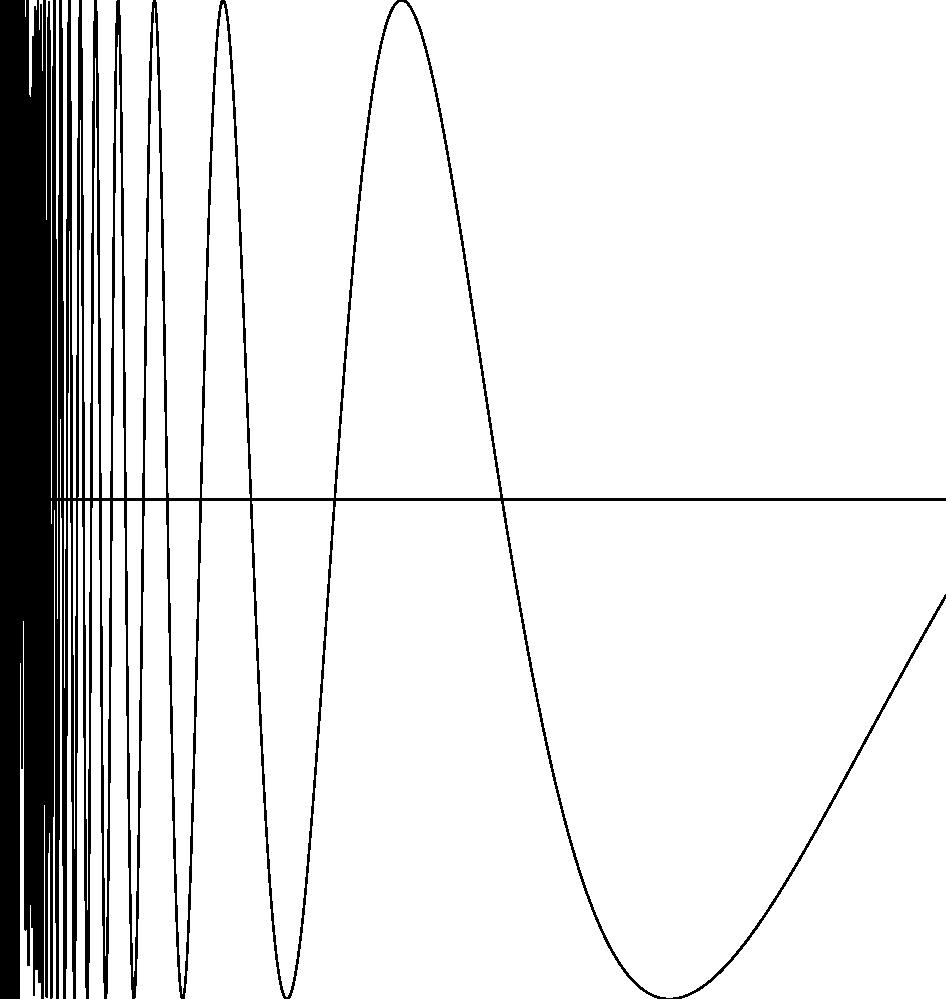
\includegraphics[width=0.7\linewidth]{sin_1_over_x.pdf}
    \end{center}
    Иначе это $\Cl$(график $\sin \frac{1}{x}$) -- связное, но не линейно связное.
\end{example}

\begin{remark}
    \

    \begin{enumerate}
        \item $A$ линейно связное, $\Cl A$ не обязательно линейно связное
        \item Компоненты линейной связности не обязательно замкнуты
        \item Отношения <<соединены путем>> -- отношения эквивалентности:
              \begin{itemize}
                  \item Рефлексивность: $x_0 \sim x_0: f(t) = x_0$
                  \item Симметричность: $f(t): f(0) = x_0, f(1) = x_1, g(t)= f(1-t): g(0) = x_1, g(1) = x_0$
                  \item Транзитивность: $f(t)$ соединяет $x_0$ и $x_1$, $g(t)$ соединяет $x_1$ и $x_2$.
                        \[h(t) = \begin{cases}
                                f(2t)   & t \in \left[0, \frac{1}{2}\right] \\
                                g(2t-1) & t \ge \frac{1}{2}
                            \end{cases}\]
              \end{itemize}
    \end{enumerate}
\end{remark}

\begin{example}
    Выпуклые множества. $A$ называется выпуклым, если для любой точки $x_0, x_1 \in A: [x_0, x_1] \subset A$.
    Такое множество линейно связно.
    \[f(t) = (1-t) x_0 + t x_1\]
    \begin{center}
        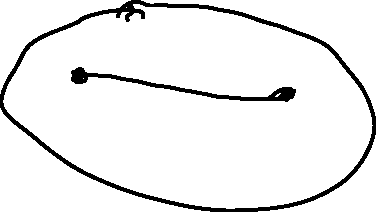
\includegraphics[width=0.5\linewidth]{convex_set.pdf}
    \end{center}
\end{example}
\begin{example}
    Звездные множества $\R^n$.
    $A$ называется звездным, если $\exists x_0 \in A: \forall x_1 \in A\ [x_0, x_1] \subset A$.
    \begin{center}
        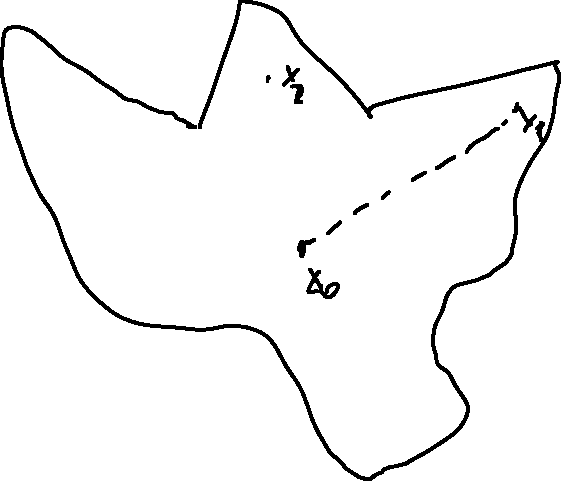
\includegraphics[width=0.5\linewidth]{star_convex_set.pdf}
    \end{center}
\end{example}

\begin{remark}
    Связность и линейная связность -- топологические свойства.
\end{remark}

\begin{theorem}[Вейерштрасса о промежуточном значении]
    $X$ -- связное пространство, $f: X \to \R$ непрерывная функция.
    $f(x_0) = a$, $f(x_1) = b$. Пусть $a \le c \le b \implies \exists x_* \in X: f(x_*) = c$
\end{theorem}
\begin{proof}
    Допустим противное: $f^{-1}(c) = \varnothing$.
    Пусть $U_1 = (-\infty, c),\ U_2 = (c, +\infty)$.
    Тогда $f^{-1}(U_1)$ и $f^{-1}(U_2)$ -- открытые непересекающиеся подмножества.
    $f^{-1}(U_1) \cup f^{-1}(U_2) = X$.
    $x_0 \in f^{-1}(U_1)$ и $x_1 \in f^{-1}(U_2)$, значит $X$ несвязно.
\end{proof}
\begin{example}
    Блин -- открытое связное ограниченное подмножество $\R^2$.
    Его можно разрезать прямой на 2 равновеликие части.
    \[
        f(t) = S_1 \quad f(-\infty) = 0 \quad f(+\infty) = S
        \implies \exists t: f(t) = S/2
    \]
    (надо доказать непрерывность, например, $f$).
    \begin{center}
        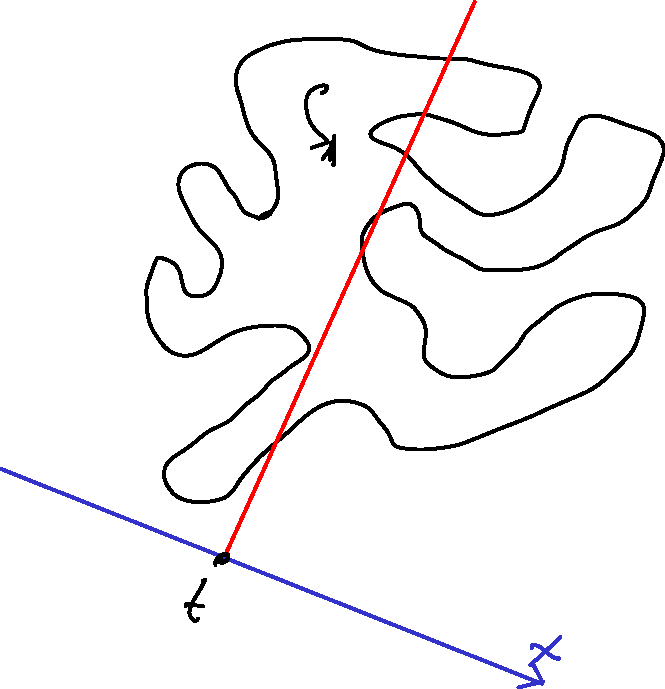
\includegraphics[width=0.7\linewidth]{pancake.pdf}
    \end{center}
\end{example}
\end{document}